% =====================================================================
%  Foto der Oberfräse mit nummerierten Bedienelementen.
%  Foto: GoRapid, Wikimedia Commons, CC BY 3.0 (siehe bilder/QUELLEN.md).
%  Koordinaten relativ zum Foto: (0,0) unten links, (1,1) oben rechts.
%  Nummern wie in der Tabelle in einweisung_Oberfraese.tex
% =====================================================================
\begin{tikzpicture}
  \node[anchor=south west, inner sep=0pt] (foto) at (0,0)
    {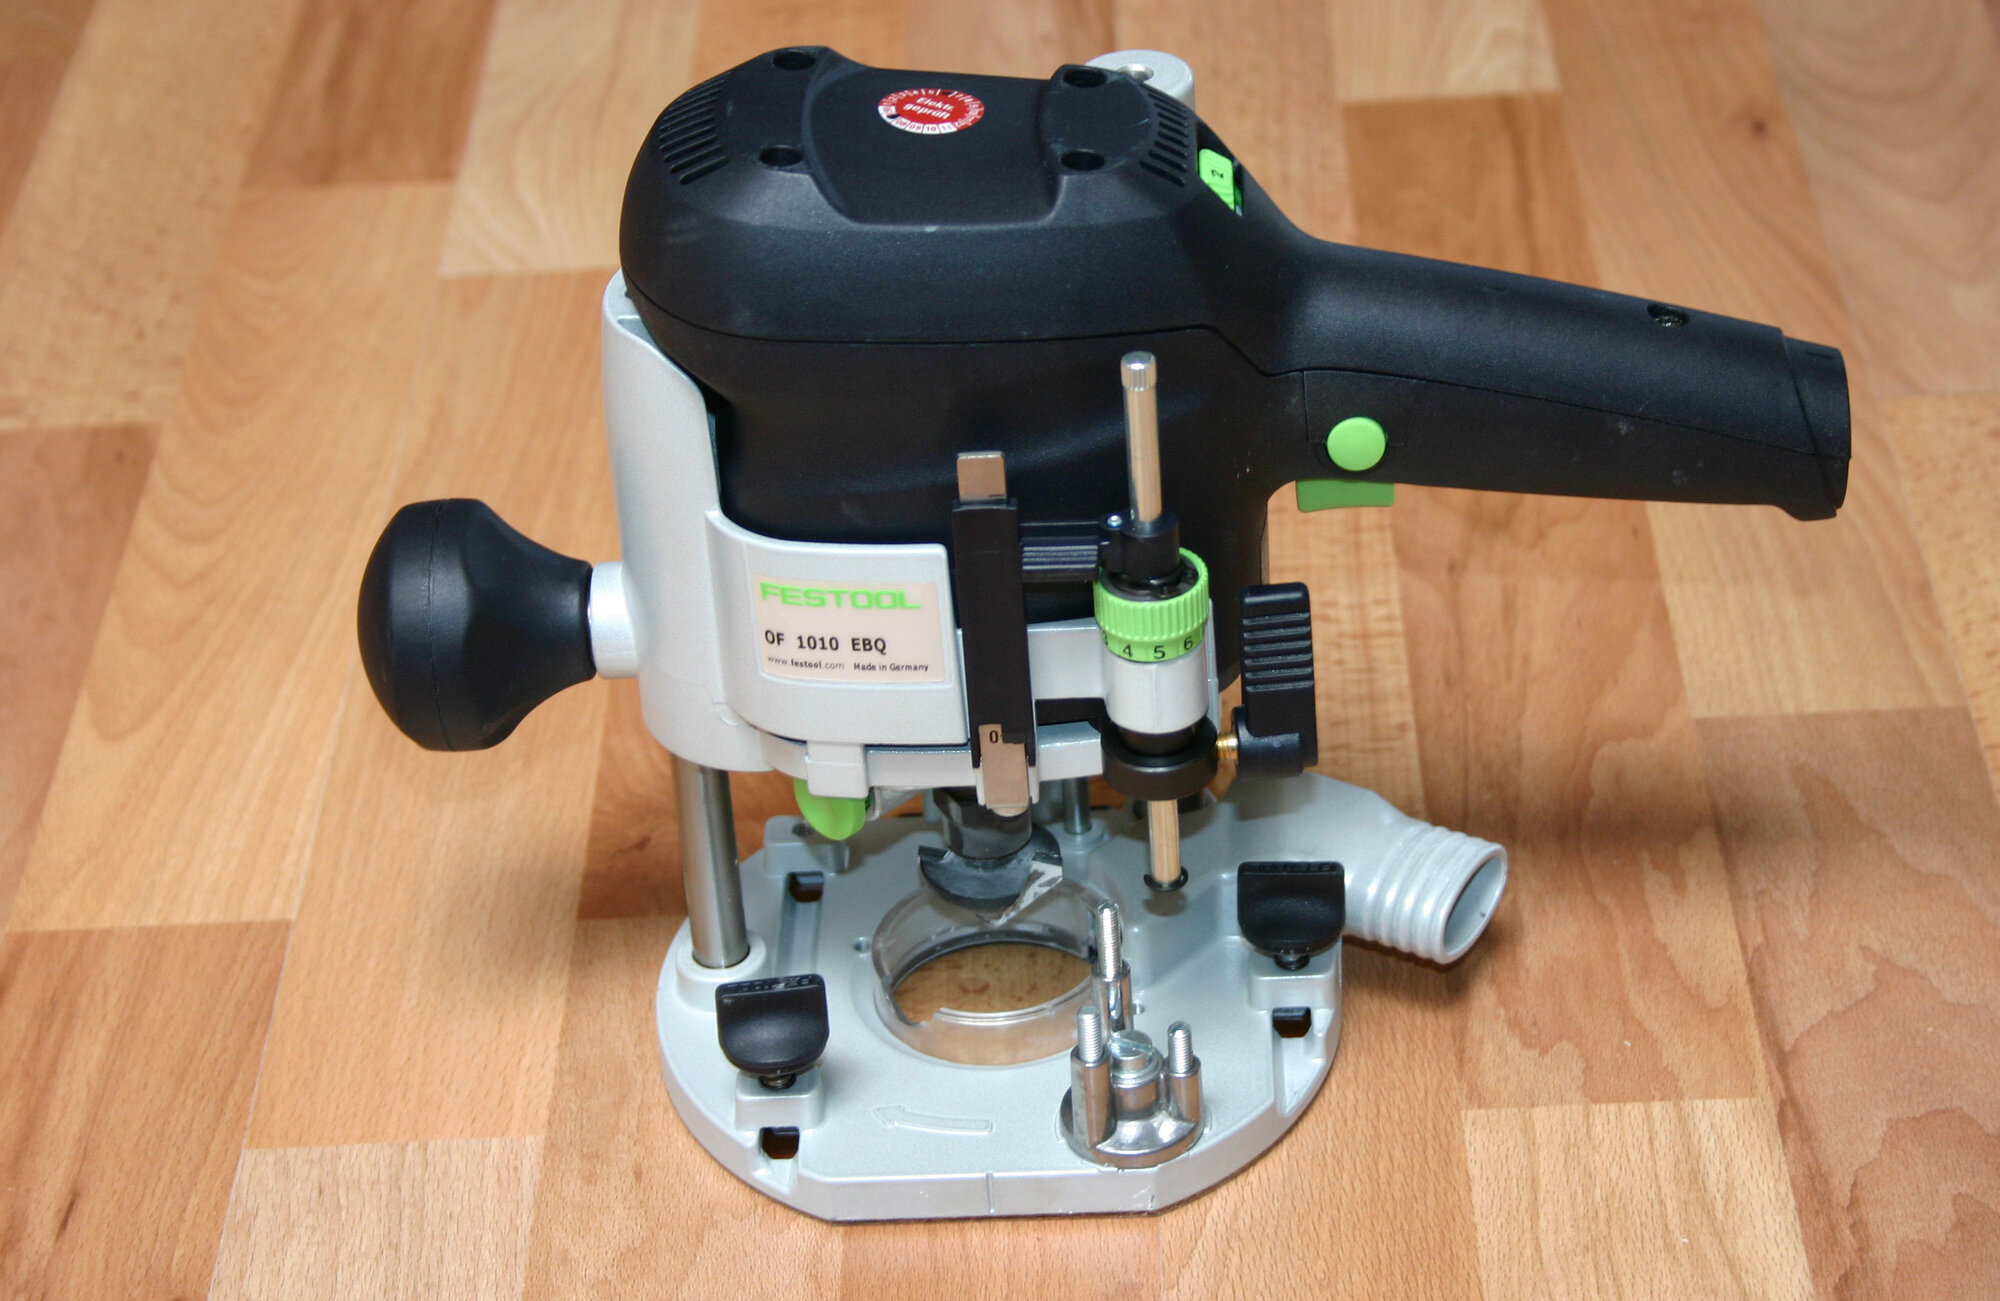
\includegraphics[width=\textwidth]{bilder/oberfraese-of1010ebq.jpg}};
  \begin{scope}[x={(foto.south east)}, y={(foto.north west)}]
    % \nr{Nummer}{Position der Nummer}{Bauteil}
    \newcommand{\nr}[3]{%
      \draw[white, line width=2pt, line cap=round] (#2) -- (#3);
      \draw[black, line width=0.8pt] (#2) -- (#3);
      \fill[black] (#3) circle[radius=0.7mm];
      \node[marke, minimum size=5.5mm, font=\small\bfseries, line width=1pt] at (#2) {#1};}
    \nr{1}{0.67,0.95}{0.608,0.868}
    \nr{2}{0.87,0.87}{0.80,0.745}
    \nr{3}{0.73,0.86}{0.677,0.655}
    \nr{4}{0.74,0.53}{0.672,0.620}
    \nr{5}{0.31,0.33}{0.412,0.388}
    \nr{6}{0.83,0.37}{0.73,0.325}
    \nr{7}{0.43,0.035}{0.466,0.141}
    \nr{8}{0.29,0.12}{0.389,0.126}
    \nr{9}{0.44,0.24}{0.492,0.336}
    \nr{10}{0.63,0.04}{0.565,0.157}
    \nr{11}{0.62,0.26}{0.582,0.36}
    \nr{12}{0.71,0.45}{0.645,0.49}
    \nr{13}{0.45,0.75}{0.566,0.556}
    \nr{14}{0.12,0.60}{0.205,0.53}
  \end{scope}
\end{tikzpicture}
